\documentclass[11pt,a4paper]{article}
\usepackage[margin=1in]{geometry}
\usepackage{graphicx}
\usepackage{hyperref}
\usepackage{xcolor}
\usepackage{listings}
\usepackage{booktabs}
\usepackage{caption}
\usepackage{float}
\usepackage{longtable}
\usepackage{tabularx}
\usepackage{verbatim}
\usepackage{makecell}
\usepackage{enumitem}
\usepackage{titlesec}
\usepackage{setspace}
\usepackage{ragged2e}
\usepackage{mdframed}
\usepackage{tikz}
\usepackage{fontspec}
\usepackage{unicode-math}
\usepackage{microtype}
\usepackage{csquotes}
\usepackage{ellipsis}

% ============================================================
% FONTS — Professional Adobe Source family (Butterick recommended)
% Source Serif 4 for body, Source Sans 3 for headings, Source Code Pro for mono
% ============================================================
\setmainfont{Source Serif 4}[
  Scale = 1.0,
  Ligatures = TeX,
  Numbers = OldStyle
]
\setsansfont{Source Sans 3}[
  Scale = 0.95,
  Ligatures = TeX
]
\setmonofont{Source Code Pro}[
  Scale = 0.84,
  Ligatures = TeX
]
\setmathfont{STIX Two Math}

% ============================================================
% COLOR PALETTE — Editorial light, restrained (non-AI)
% Warm paper, soft ink, deep navy + muted slate. Based on
% Butterick: "good typography is 90% good fonts + restraint"
% ============================================================
\definecolor{ink}{HTML}{1A1A1E}          % Soft black, not pure #000
\definecolor{paper}{HTML}{FFFEFC}        % Warm white
\definecolor{cardbg}{HTML}{F8F9FA}       % Light card
\definecolor{border}{HTML}{E5E7EB}       % Subtle border
\definecolor{accent}{HTML}{14365D}       % Deep navy — headings, links
\definecolor{accent2}{HTML}{7A2424}      % Deep oxblood — secondary
\definecolor{success}{HTML}{1B6B4A}      % Muted forest
\definecolor{warn}{HTML}{8A6D00}         % Muted amber
\definecolor{danger}{HTML}{8B1A1A}       % Muted brick
\definecolor{fg}{HTML}{1A1A1E}
\definecolor{fgmuted}{HTML}{6B7280}      % Slate gray
\definecolor{codebg}{HTML}{F3F4F6}       % Light gray code
\definecolor{linkcolor}{HTML}{14365D}

\pagecolor{paper}
\color{ink}

% ============================================================
% HYPERLINKS
% ============================================================
\hypersetup{
    colorlinks=true,
    linkcolor=accent,
    urlcolor=accent2,
    citecolor=success,
    pdfauthor={Aayush Bankar},
    pdftitle={CVE-2026-46242 Deep Dive: Root on Linux, DoS on Android},
    pdfsubject={Kernel exploitation research},
    pdfkeywords={CVE-2026-46242, Bad Epoll, kernel exploitation, UAF, Android, ARM64},
    bookmarks=true,
    bookmarksnumbered=true,
    bookmarksopen=true,
}

% ============================================================
% LISTINGS — Modern code blocks
% ============================================================
\definecolor{keyword}{HTML}{7A2424}
\definecolor{string}{HTML}{1B4F72}
\definecolor{comment}{HTML}{6B7280}
\definecolor{type}{HTML}{14365D}
\definecolor{number}{HTML}{6B7280}

\lstset{
    backgroundcolor=\color{codebg},
    basicstyle=\ttfamily\footnotesize\color{ink},
    keywordstyle=\color{keyword}\bfseries,
    stringstyle=\color{string},
    commentstyle=\color{comment}\itshape,
    numberstyle=\tiny\color{fgmuted},
    identifierstyle=\color{ink},
    showstringspaces=false,
    breaklines=true,
    breakatwhitespace=false,
    frame=single,
    framesep=6pt,
    framerule=1pt,
    rulecolor=\color{border},
    xleftmargin=1.4em,
    xrightmargin=1.4em,
    framexleftmargin=8pt,
    framexrightmargin=8pt,
    tabsize=2,
    columns=fullflexible,
    keepspaces=true,
    showspaces=false,
    showtabs=false,
    numbers=left,
    numbersep=10pt,
    stepnumber=1,
    firstnumber=auto,
    captionpos=b,
    abovecaptionskip=0.6em,
    belowcaptionskip=0.6em,
    escapeinside={(*@}{@*)},
    morekeywords={struct,static,inline,const,volatile,register,typeof,__attribute__,
      WRITE_ONCE,READ_ONCE,spin_lock,spin_unlock,hlist_del_rcu,hlist_add_head_rcu,
      kmalloc,kfree,epoll_ctl,epoll_create1,close,msgsnd,msgrcv,percpu_counter_dec,
      commit_creds,prepare_kernel_cred,SWAPGS,SWAPGS_RESTORE_REGS_AND_RETURN_TO_USERMODE},
    morekeywords=[2]{int,long,short,char,void,unsigned,signed,size_t,ssize_t,uint8_t,uint16_t,uint32_t,uint64_t},
    keywordstyle=[2]\color{type}\bfseries,
}

% ============================================================
% SECTION STYLING — Editorial, restrained (Butterick: hierarchy via size/weight)
% ============================================================
\titleformat{\section}
  {\LARGE\bfseries\color{accent}\sffamily}
  {\thesection}{0.7em}{}
  [{\vspace{0.4em}\color{border}\titlerule[0.6pt]}]

\titleformat{\subsection}
  {\Large\bfseries\color{ink}\sffamily}
  {\thesubsection}{0.6em}{}

\titleformat{\subsubsection}
  {\large\bfseries\color{ink}\sffamily}
  {\thesubsubsection}{0.6em}{}

\titlespacing{\section}{0pt}{2.2em plus 0.4em}{0.9em plus 0.2em}
\titlespacing{\subsection}{0pt}{1.6em plus 0.3em}{0.6em plus 0.2em}
\titlespacing{\subsubsection}{0pt}{1.2em plus 0.2em}{0.5em plus 0.1em}

% ============================================================
% CUSTOM ENVIRONMENTS — Subtle, editorial callouts (no neon)
% Left-rule style, like Bringhurst / Tufte marginalia
% ============================================================

% Disclosure / important box — left accent bar, not full border
\newmdenv[
  backgroundcolor=cardbg,
  linecolor=accent,
  linewidth=3pt,
  topline=false,
  bottomline=false,
  rightline=false,
  leftline=true,
  innerleftmargin=14pt,
  innerrightmargin=12pt,
  innertopmargin=10pt,
  innerbottommargin=10pt,
  skipabove=1.1em,
  skipbelow=1.1em,
]{calloutbox}

% Pull quote — thin left rule, italic
\newmdenv[
  backgroundcolor=paper,
  linecolor=border,
  linewidth=1.2pt,
  topline=false,
  bottomline=false,
  rightline=false,
  leftline=true,
  innerleftmargin=14pt,
  innerrightmargin=12pt,
  innertopmargin=8pt,
  innerbottommargin=8pt,
  skipabove=0.9em,
  skipbelow=0.9em,
]{pullquote}

% Warning / danger box — oxblood left rule
\newmdenv[
  backgroundcolor=cardbg,
  linecolor=danger,
  linewidth=3pt,
  topline=false,
  bottomline=false,
  rightline=false,
  leftline=true,
  innerleftmargin=14pt,
  innerrightmargin=12pt,
  innertopmargin=10pt,
  innerbottommargin=10pt,
  skipabove=1em,
  skipbelow=1em,
]{dangerbox}

% Success box — forest left rule
\newmdenv[
  backgroundcolor=cardbg,
  linecolor=success,
  linewidth=3pt,
  topline=false,
  bottomline=false,
  rightline=false,
  leftline=true,
  innerleftmargin=14pt,
  innerrightmargin=12pt,
  innertopmargin=10pt,
  innerbottommargin=10pt,
  skipabove=1em,
  skipbelow=1em,
]{successbox}

% Code callout inline
\newcommand{\inlinecode}[1]{\colorbox{codebg}{\ttfamily\small\color{keyword}#1}}

% Icon macros - text-based since DejaVu Sans lacks emoji glyphs
\newcommand{\githubicon}{[GitHub]}
\newcommand{\linkedinicon}{[LinkedIn]}
\newcommand{\targeticon}{[TARGET]}
\newcommand{\toolicon}{[TOOL]}

% ============================================================
% TABLES — Editorial styling
% ============================================================
\colorlet{tablehead}{accent}
\colorlet{tableheadfg}{paper}
\colorlet{tablerow}{cardbg}
\colorlet{tableborder}{border}

% Typography refinements
\setlength{\emergencystretch}{2.5em}
\tolerance=900
\hyphenpenalty=350
\exhyphenpenalty=350
\frenchspacing
\widowpenalty=10000
\clubpenalty=10000
\displaywidowpenalty=10000
\captionsetup{font={small,sf,color=fgmuted}, labelfont={bf,color=accent}, justification=raggedright, singlelinecheck=false}
\AtBeginEnvironment{tabular}{\sffamily\small}
\AtBeginEnvironment{tabularx}{\sffamily\small}

% ============================================================
% DOCUMENT
% ============================================================
\begin{document}

% ============================================================
% COVER PAGE — Big, bold, minimal
% ============================================================
\thispagestyle{empty}
\vspace*{4cm}
\begin{center}
  {\Huge\bfseries\color{fg} CVE-2026-46242 Deep Dive}\\[0.4em]
  {\Large\color{accent} Root on Linux, DoS on Android}\\[2.5em]
  
  {\large\color{fgmuted} Aayush Bankar}\\[0.3em]
  {\color{fgmuted} Cybersecurity Analyst @ CypherMatrix}\\[2em]
  
  \begin{tabular}{ll}
    \color{fgmuted}Tier 1: & \color{accent}\texttt{github.com/Aayushbankar/bad-epoll-lab} \\
    \color{fgmuted}Tier 2: & \color{accent2}\texttt{github.com/Aayushbankar/bad\_epoll\_ab\_tier2} \\
  \end{tabular}\\[2em]
  
  {\color{fgmuted} Original vuln by \textbf{Jaeyoung Chung} via Google kernelCTF}\\[2em]
  
  {\color{fgmuted} August 2026}\\[1em]
  {\color{fgmuted} Independent reproduction \& exploitability research}\\
  {\color{fgmuted} No 0-days disclosed}
\end{center}
\vfill
{\color{fgmuted}\footnotesize Built with \texttt{xelatex} | Fonts: Source Serif 4 + Source Sans 3 + Source Code Pro}

\newpage
\tableofcontents
\newpage

% ============================================================
% SCOPE & ATTRIBUTION
% ============================================================
\section{Scope \& Attribution}

\begin{calloutbox}
\noindent\textbf{\large [TARGET] Original Discovery \& Exploit}\\
CVE-2026-46242 (\enquote{Bad Epoll}, CVSS 7.8) was discovered, analyzed, and exploited by \textbf{Jaeyoung Chung} (\texttt{github.com/J-jaeyoung/bad-epoll}) via Google's kernelCTF. Patched upstream in \texttt{a6dc643c693} (v6.11 / v7.1-rc1).

\vspace{1em}
\noindent\textbf{\large [TOOL] This Project's Contribution}
\begin{enumerate}
  \item \textbf{Tier 1 (x86\_64/QEMU):} Independent reproduction, GCC 16 toolchain port, database regeneration, runtime verification of the kernelCTF chain.
  \item \textbf{Tier 2 (ARM64 Android 14 GKI):} Original portability/exploitability research --- did the primitive survive PAC, BTI, kCFI, MTE, slab isolation? \textbf{Documented negative result: DoS-only.}
\end{enumerate}
\end{calloutbox}

\begin{dangerbox}
\noindent\textbf{\large [!] Tier 2 Test Methodology Disclosure}

The Tier 2 assessment did \textbf{not} run against a stock/production Android kernel.

\textbf{Stock Android GKI 6.1.23 (base commit \texttt{7e35917775b8}) is NOT vulnerable to CVE-2026-46242} --- the introducing commit \texttt{58c9b016e128} (v6.4-rc1) is absent from the 6.1 branch. This matches discoverer Jaeyoung Chung's own affected-version statement (bug introduced in v6.4, so Pixel 8 et al. are safe).

To study what Android's mitigation stack does to \textit{this} primitive, we \textbf{deliberately cherry-picked the 6.1.y backport \texttt{a1f93804449d} into GKI 6.1.23} to build a vulnerable test kernel. Every Tier 2 result below (0/102,740 natural race hits, 21 dead ends, DoS-only) is a \textbf{portability/mitigation study of a synthetic backported-vulnerable kernel} --- \textbf{not} a finding about any production Android device.

Correct framing: \enquote{If CVE-2026-46242 existed on GKI 6.1, would Android's mitigations stop it?} --- \textbf{not} \enquote{We tested a real vulnerable Android kernel.}
\end{dangerbox}

\newpage

% ============================================================
% EXECUTIVE SUMMARY — Verdict AMBER
% ============================================================
\section{Executive Summary}
\label{sec:executive}

\textbf{Verdict: AMBER — DoS-only negative result, scientifically defensible (not a failure).}

The UAF is \textbf{real and 100\% reproducible with debugger assistance} (hardware watchpoint VER-026) and \texttt{msg\_msg} reclaim of freed \texttt{struct eventpoll} in \texttt{kmalloc-192} is \textbf{reliable} (VER-027). However the race is \textbf{not naturally schedulable}: 0/102,740 unaided attempts across NAT-001 and NAT-005 (VER-034/039). All four exploitation chains are structurally dead (21 dead ends); the only remaining primitive is a fixed NULL write at offset 160, which the EXP-016 audit proves is DoS-only on this config. \textbf{Recommendation:} 2-week timebox on physical ARM64 hardware to test timing-widening; if 0 hits in $\sim$1M iterations, conclude DoS-only. Full evidence in \texttt{tier2/docs/VERIFICATION\_LEDGER.md} (42 entries), \texttt{DEAD\_ENDS\_REGISTER.md} (21), \texttt{ASSUMPTIONS\_REGISTER.md} (42).

\newpage

% ============================================================
% INTRODUCTION
% ============================================================
\section{Introduction}

Every Linux process handling network connections, file descriptors, or event loops uses \texttt{epoll}. nginx, Node.js, Android's SurfaceFlinger, Binder --- all depend on it. When a UAF lands here, blast radius = everything.

\textbf{CVE-2026-46242 (Bad Epoll)} is a race in the kernel's \texttt{epoll} implementation that frees a critical structure while another thread is still writing to it.

\begin{itemize}
  \item \textbf{x86\_64:} Ported \& reproduced the kernelCTF chain $\to$ working root shell (\texttt{UID: 0}).
  \item \textbf{ARM64 Android GKI 6.1 (backported-vuln build):} 21 dead ends, \textbf{0/102,740} natural race hits, verdict = \textbf{DoS only} (on synthetic build, not stock Android).
\end{itemize}

This is the full technical story: vuln mechanics, working x86\_64 chain, systematic ARM64 assessment, every failed chain \& why, what Android's mitigations actually stop.

% ============================================================
% CVE BASICS TABLE
% ============================================================
\section{CVE-2026-46242: The Basics}

\begin{table}[H]
\centering
\caption{CVE-2026-46242 Summary}
\label{tab:cve}
\begin{tabularx}{\textwidth}{>{\bfseries\color{accent}}l X}
\toprule
\textbf{Field} & \textbf{Value} \\
\midrule
CVE & CVE-2026-46242 (CVSS 7.8) \\
Name & Bad Epoll \\
Class & Use-After-Free (race condition) \\
Subsystem & \inlinecode{fs/eventpoll.c} \\
Discoverer & Jaeyoung Chung (\texttt{github.com/J-jaeyoung/bad-epoll}) via kernelCTF \\
Introduced & v6.4-rc1 (\texttt{58c9b016e128}) \\
Patched & v6.11 / v7.1-rc1 (\texttt{a6dc643c693}) \\
Affected & Linux 6.4--6.10.x, Android GKI $\ge$ 6.4. \textbf{GKI 6.1 NOT affected} (commit \texttt{58c9b016e128} absent). \\
Impact & LPE to root (x86\_64 kernelCTF); DoS-only on backported-vuln GKI 6.1 test build. \\
\bottomrule
\end{tabularx}
\end{table}

\begin{calloutbox}
\noindent\textbf{\large Evidence-First Methodology}
\begin{itemize}
  \item \textbf{42} verification entries mapped to GDB hardware watchpoints / static audits
  \item \textbf{3} retracted claims (VER-010, 029, 030) --- kept visible with reasons
  \item \textbf{21} dead ends with killing evidence
  \item \textbf{42} assumptions tracked (validated $\to$ falsified)
  \item All raw evidence (GDB logs, serial output, disassembly) in repos
\end{itemize}
Full chain: \texttt{VERIFICATION\_LEDGER.md}, \texttt{DEAD\_ENDS\_REGISTER.md}, \texttt{ASSUMPTIONS\_REGISTER.md}
\end{calloutbox}

\newpage

% ============================================================
% ENVIRONMENT & REPRODUCIBILITY
% ============================================================
\section{Environment \& Reproducibility}
\label{sec:env}

\subsection{Tier 1 — x86\_64 (Fedora 44, Linux 6.12.67, QEMU)}
\begin{itemize}
  \item Host: Fedora 44, x86\_64, GCC 16.1.1, QEMU
  \item Kernel: 6.12.67 compiled with DWARF BTF, \texttt{nokaslr} (KASLR disabled for determinism), base \texttt{0xffffffff81000000}
  \item Target DB: \texttt{lts-6.12.67} rebuilt via \texttt{rp++} + \texttt{angrop} (patched \texttt{PicklingError} in \texttt{SpecialMem})
  \item Offsets (GDB-mapped, vs Google defaults): \texttt{task\_struct.comm} 1840 (was 1928), \texttt{files} 1896 (1984), \texttt{children} 1384 (1472), \texttt{sibling} 1400 (1488)
  \item Verified gadgets: \texttt{POP\_RDI\_RET 0x1600ea0} (\texttt{0xffffffff81600ea0}: \texttt{pop rdi; jmp \_\_x86\_return\_thunk}), \texttt{POP\_RET 0x42010}, \texttt{\_\_x86\_return\_thunk 0x20d6e70}
  \item Race tuning: \texttt{RACE\_DUP\_CLOSE\_ITERS 20} (was 250), \texttt{RACE\_AHEAD\_HI 10000ns} (4000ns), timeout 600s
  \item Rootfs: custom \texttt{initramfs.cpio} with busybox, \texttt{/init} mounts \texttt{/proc,/sys}, payload at \texttt{exploit/tier1/rootfs\_debug/bin/exploit}
  \item Evidence: \texttt{qemu\_output.log} (Win! UID 0), \texttt{target\_db.kxdb} SHA256 \texttt{63542e7f...}, exploit SHA256 \texttt{95cd9f36...}
\end{itemize}
Rebuild: \texttt{make} kernel $\to$ \texttt{start\_qemu.sh} $\to$ \texttt{tail -f qemu\_output.log}. Gadget DB must match exact \texttt{vmlinux}; see \texttt{knowledge/02\_projects/bad-epoll/01\_tier1/02\_env\_rebuild\_guide.md} and \texttt{03\_offsets\_layout.md}.

\subsection{Tier 2 — Android ARM64 GKI (QEMU aarch64 + GDB)}
\begin{itemize}
  \item Base: Android 14 GKI 6.1.23 @ \texttt{7e35917775b8}, stock \textbf{NOT vulnerable} (no \texttt{58c9b016e128}); test kernel = base + cherry-picked 6.1.y backport \texttt{a1f93804449d} (deliberately backported-vulnerable)
  \item Artifacts: \texttt{tier2/android/artifacts/Image}, \texttt{vmlinux} (285 MB, debug\_info, 98575 symbols via \texttt{System.map}), \texttt{initramfs.cpio} (BusyBox)
  \item Toolchain: \texttt{aarch64-linux-gnu-gcc} (static), \texttt{qemu-system-aarch64 -nographic -s -S}, \texttt{gdb-multiarch}, \texttt{gdb\_race\_test.py} (sync\_flag + \texttt{dmb sy; b .} patch)
  \item Config: \texttt{PREEMPT\_VOLUNTARY}, \texttt{CONFIG\_PREEMPT\_DYNAMIC=y} (default voluntary), \texttt{SLAB\_ACCOUNT} on, \texttt{CONFIG\_MEMCG=n}, \texttt{CONFIG\_UNUSED\_KSYMS\_WHITELIST} patched
  \item Reclaim: \texttt{msg\_msg} 144B payload in \texttt{kmalloc-192}, marker \texttt{0xdead000000000000} at user byte 88 (offset 136) verified via GDB dump
\end{itemize}
Runbook: \texttt{tier2/docs/TIER2\_MANUAL\_RUNBOOK.md} (redacted, now at \texttt{tier2/docs/TIER2\_MANUAL\_RUNBOOK.md}); 2-min demo \texttt{test\_gdb.sh} + \texttt{gdb -x gdb\_race\_test.py vmlinux}.

\newpage

% ============================================================
% THE VULNERABILITY
% ============================================================
\section{The Vulnerability: Race in the Heart of I/O}

The bug lives in \texttt{\_\_ep\_remove()} vs \texttt{eventpoll\_release()} --- concurrent execution when nested \texttt{epoll} fds are closed from different threads.

\textbf{Setup:} Two epoll instances --- outer watches inner.

\begin{lstlisting}[language=C, caption=Nested epoll setup, label=lst:nested]
int outer = epoll_create1(0);
int inner = epoll_create1(0);
epoll_ctl(outer, EPOLL_CTL_ADD, inner, &ev);  // inner watched by outer
\end{lstlisting}

\textbf{Thread A} (\texttt{close(outer)}) $\to$ \texttt{\_\_ep\_remove()} clears backpointer:

\begin{lstlisting}[language=C, caption=Thread A clears backpointer]
WRITE_ONCE(file->f_ep, NULL);  // Clears inner file's epoll backpointer
\end{lstlisting}

\textbf{Thread B} (\texttt{close(inner)}) $\to$ \texttt{\_\_fput()} $\to$ \texttt{eventpoll\_release()} checks locklessly:

\begin{lstlisting}[language=C, caption=Thread B lockless fast path]
if (!file_has_epoll(f))   // Reads f_ep --- sees NULL from Thread A
    return;                // Skips epoll cleanup entirely
\end{lstlisting}

Thread B sees \texttt{NULL}, assumes no epoll refs, \textbf{frees the \texttt{struct eventpoll}} (inner fd). Memory returns to \texttt{kmalloc-192}.

Thread A continues \texttt{\_\_ep\_remove()}:

\begin{lstlisting}[language=C, caption=Thread A UAF write]
hlist_del_rcu(&epi->fllink);  // Writes to inner_epoll->refs at offset 160
\end{lstlisting}

\textbf{8-byte NULL write at offset 0xA0 (160) of already-freed \texttt{struct eventpoll}.} This is the UAF.

\begin{figure}[H]
\centering
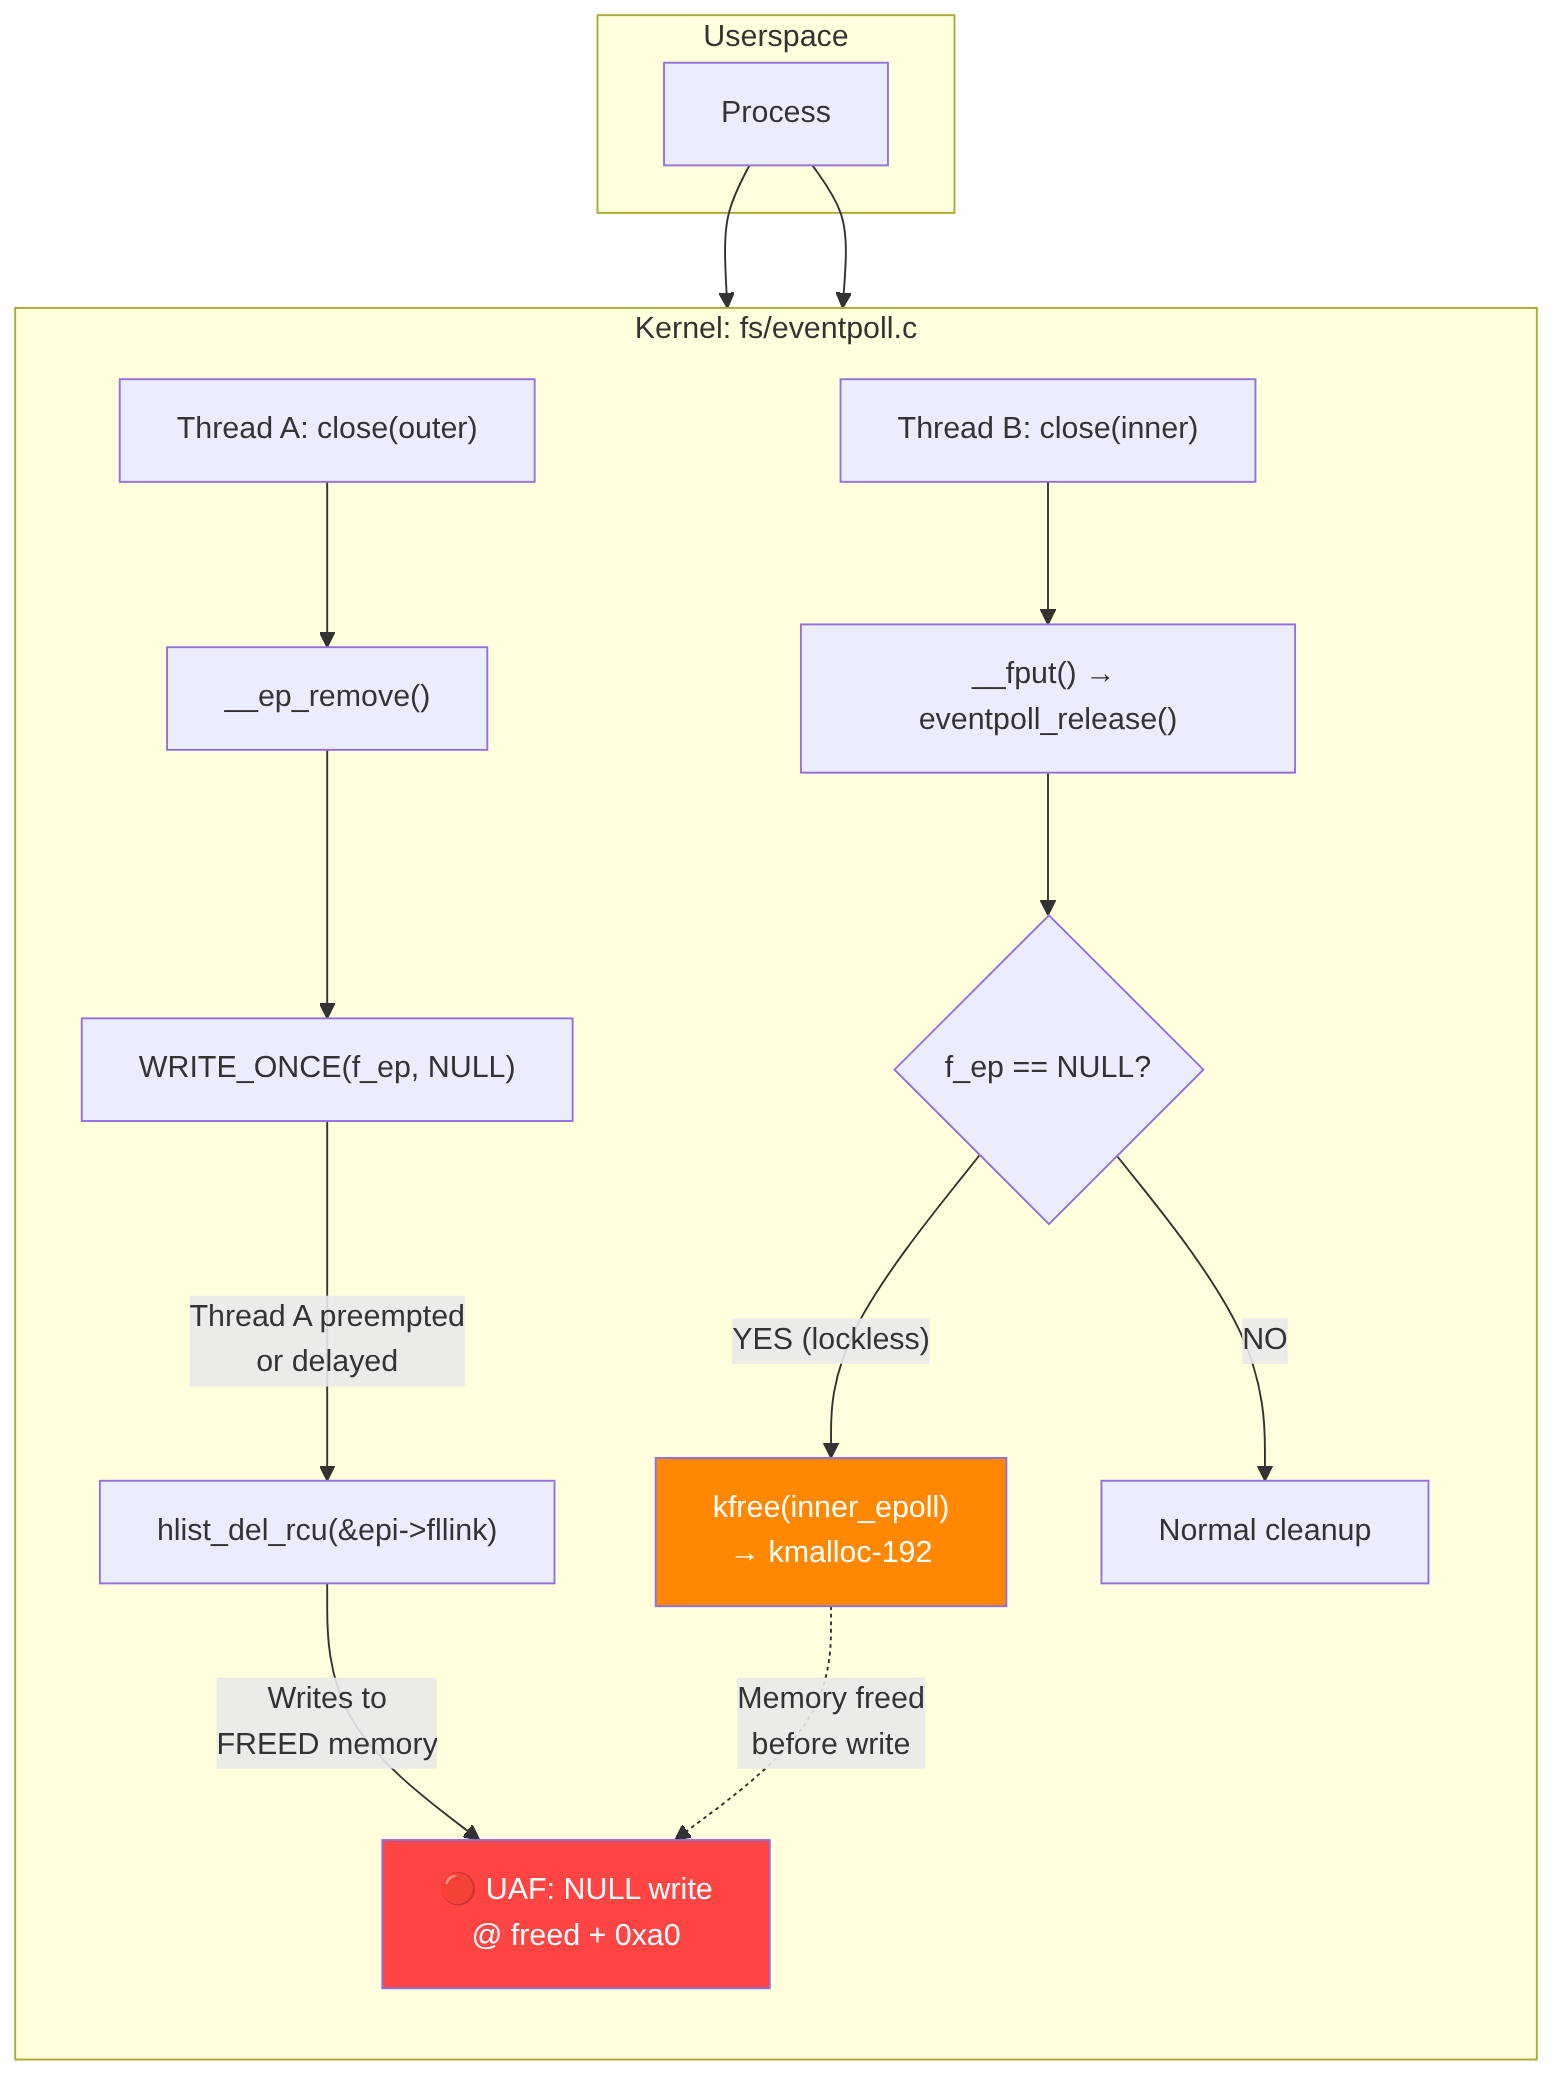
\includegraphics[width=\textwidth]{assets/diagram-01.png}
\caption{Attack Surface --- Userspace to Kernel UAF}
\end{figure}

\newpage

% ============================================================
% STRUCT EVENTPOLL
% ============================================================
\section{struct eventpoll: The Victim Object}

\texttt{struct eventpoll} = 176 bytes $\to$ \texttt{kmalloc-192}. Field at offset 160 (\texttt{refs}, \texttt{struct hlist\_head}) is the UAF target:

\begin{verbatim}
struct eventpoll (176 bytes → kmalloc-192)
┌──────────────────────────────────────────────────┐
│ 0x00: wait_queue_head_t wq            (24 B)     │
│ 0x18: wait_queue_head_t poll_wait     (24 B)     │
│ 0x30: struct list_head rdllist        (16 B)     │
│ 0x40: struct rb_root_cached rbr       (16 B)     │
│ 0x50: struct epitem *ovflist          (8  B)     │
│ 0x58: struct wakeup_source *ws        (8  B)     │
│ 0x60: struct user_struct *user        (8  B)     │
│ 0x68: struct file *file               (8  B)     │
│ 0x70: ... (misc)                      (48 B)     │
│ 0xA0: struct hlist_head refs ← UAF WRITE         │ ← offset 160
│ 0xA8: ... (remaining)               (8  B)       │
│ 0xB0: end                              (176 B)   │
└──────────────────────────────────────────────────┘
\end{verbatim}

When freed to \texttt{kmalloc-192}, attacker sprays \texttt{msg\_msg} (SysV \texttt{msgsnd} 144B user data). \texttt{msg\_msg} header = 0x00--0x2F (48B), attacker payload = 0x30--0xBF. UAF NULL write at 0xA0 lands \textbf{inside attacker payload} --- zeroes 8 bytes of their own message, no kernel pointer corruption.

\begin{figure}[H]
\centering
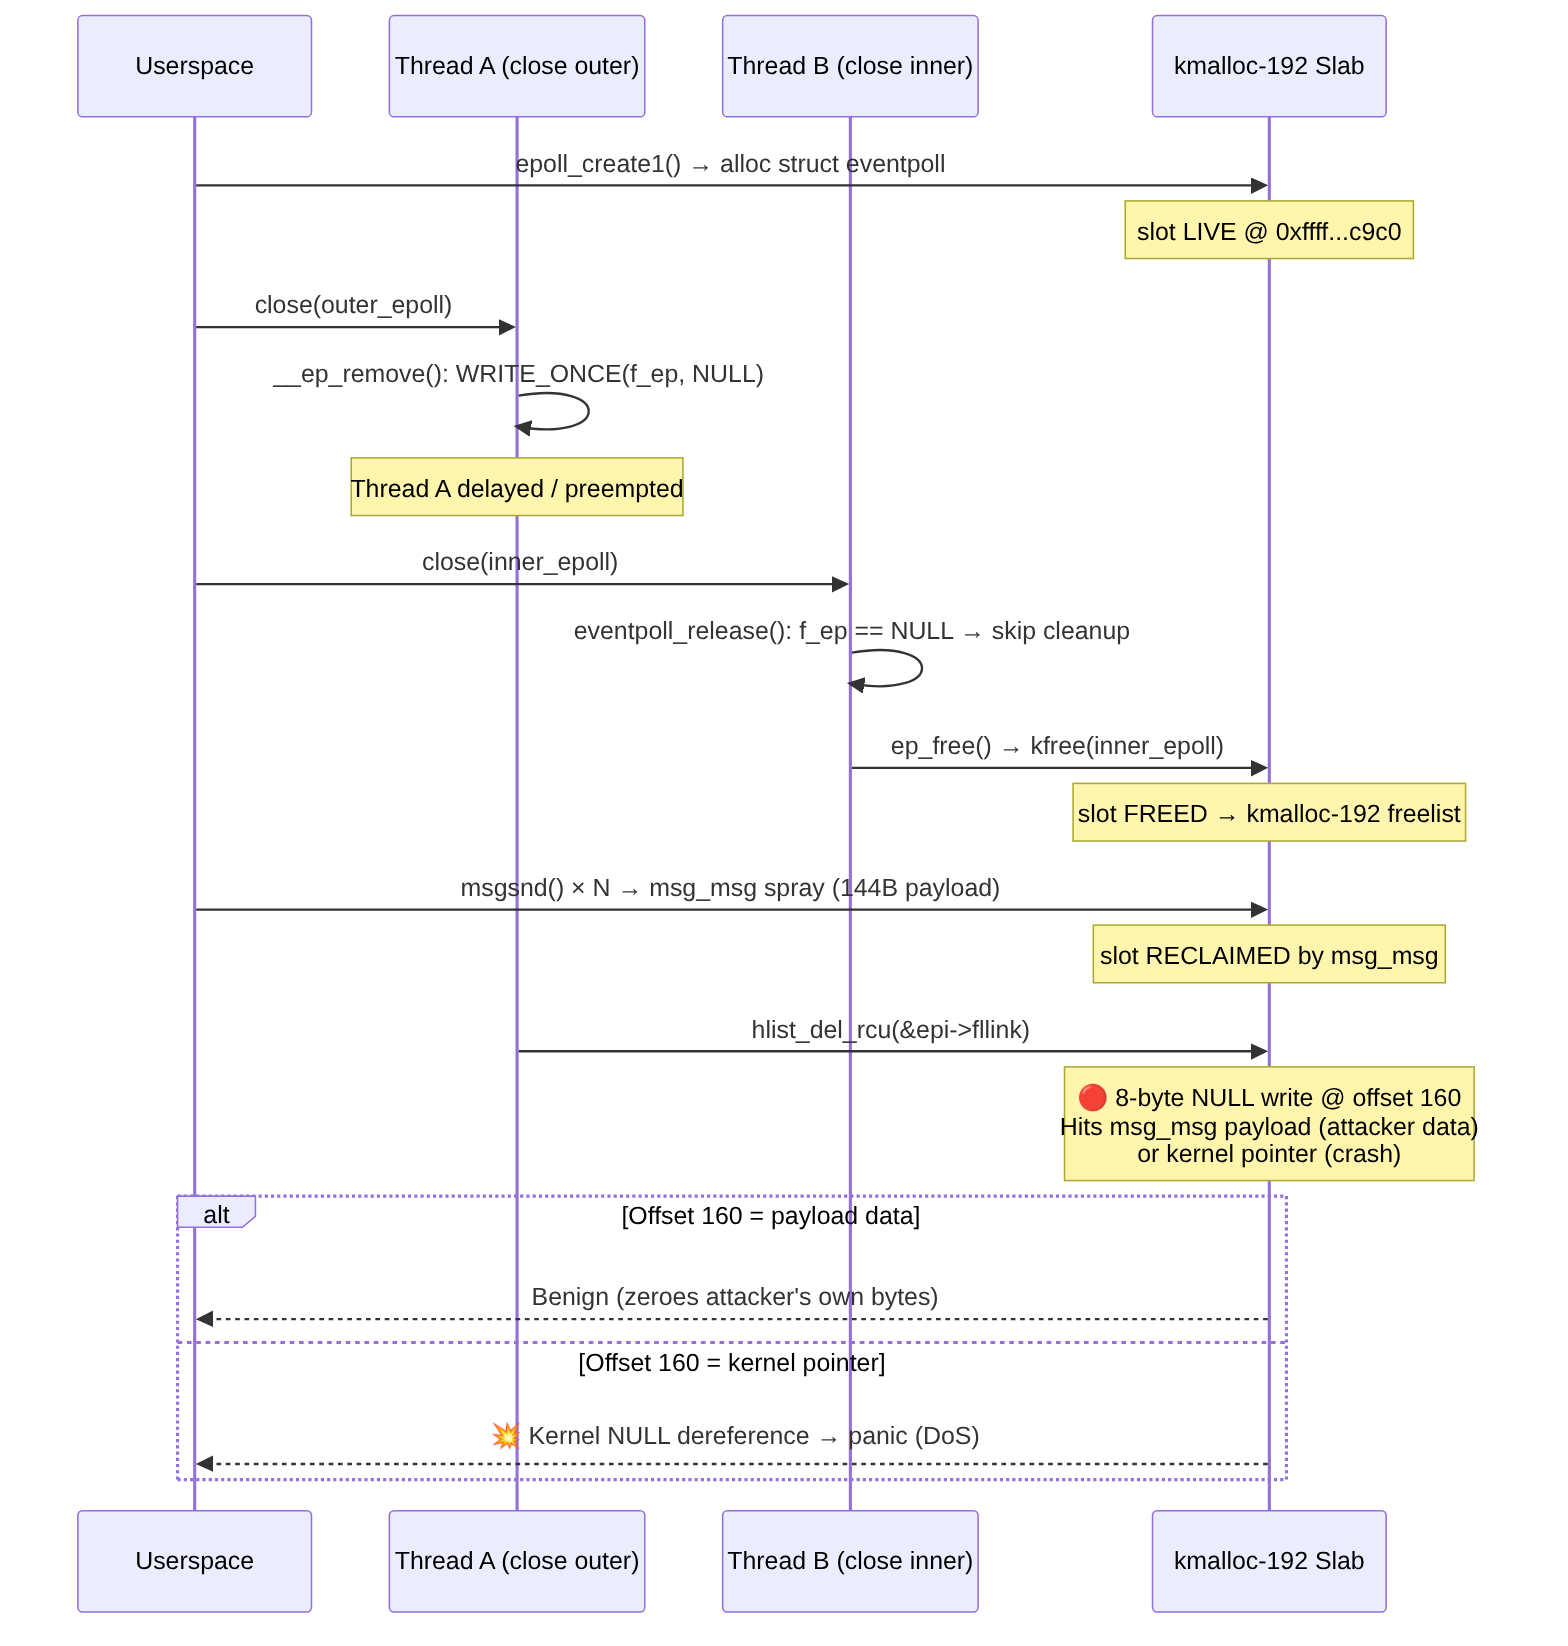
\includegraphics[width=\textwidth]{assets/diagram-02.png}
\caption{Race Timeline --- Alloc $\to$ Free $\to$ Reclaim $\to$ UAF}
\end{figure}

\newpage

% ============================================================
% TIER 1
% ============================================================
\section{Tier 1: Root on x86\_64}

\textbf{Env:} Fedora 44, Linux 6.12.67 (GCC 16.1.1), QEMU + SMEP/SMAP/KPTI.

Jaeyoung Chung's kernelCTF exploit targets \texttt{struct epitem} (120B, \texttt{eventpoll\_epi} cache on newer kernels, cross-cacheable on COS target) + \texttt{struct file}, not \texttt{struct eventpoll}.

\begin{figure}[H]
\centering
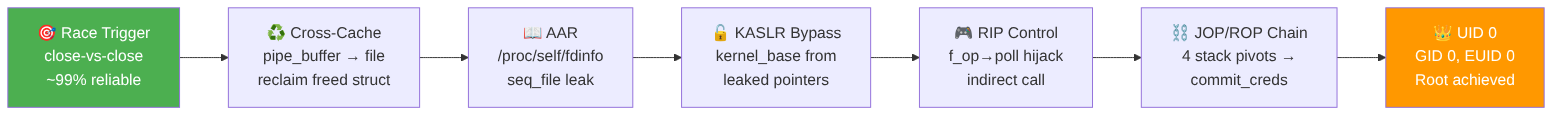
\includegraphics[width=\textwidth]{assets/diagram-03.png}
\caption{Tier 1 Exploitation Chain}
\end{figure}

\textbf{Stage 1 --- Race:} Two threads race \texttt{close()} on nested epoll FDs. $\sim$99\% success after tuning.

\textbf{Stage 2 --- Cross-cache:} Freed \texttt{struct file} reclaimed via \texttt{pipe\_buffer} spray $\to$ attacker controls \texttt{f\_op} / \texttt{f\_inode}.

\textbf{Stage 3 --- AAR:} Forge \texttt{f\_inode} $\to$ \texttt{/proc/self/fdinfo} (\texttt{seq\_file}) $\to$ leak \texttt{task\_struct} $\to$ KASLR base.

\textbf{Stage 4 --- RIP control:} Overwrite \texttt{file->f\_op->poll} $\to$ \texttt{poll()} triggers hijack.

\textbf{Stage 5 --- JOP/ROP:} 4 stack pivots via \texttt{\_\_x86\_indirect\_call\_thunk\_rdi} $\to$ RSP onto mmap'd page $\to$ \texttt{commit\_creds(\&init\_cred)} $\to$ \texttt{SWAPGS} return $\to$ \texttt{UID 0}.

\begin{verbatim}
cross-cache ok
kernel_base=ffffffff81000000
task=ffff8880...
READY_FOR_GDB
Win! UID: 0, GID: 0, EUID: 0
\end{verbatim}

\begin{pullquote}
\noindent\textbf{[IDEA] The Offset Desync Breakthrough}
Initial crash: Supervisor Write Fault at \texttt{0xffffffff810001bd} (dead padding). Root cause: upstream \texttt{target\_db.kxdb} built for Google COS kernel. GCC 16 vs Clang 12 shifts every gadget offset. Fix: regenerate DB with \texttt{rp++} + \texttt{angrop} on local \texttt{vmlinux} --- required patching \texttt{PicklingError} in \texttt{angrop} (nested \texttt{SpecialMem} class couldn't pickle).
\end{pullquote}

\textbf{Remaining:} Userland return leaves RSP misaligned $\to$ \texttt{execve("/bin/sh")} SIGSEGV. PID 1 \texttt{/init} panics kernel. Escalation proven (UID 0), shell unstable. Post-exploitation issue, not primitive failure.

\subsection{Tier 1 Constants \& Offsets}
Full reference at \texttt{knowledge/02\_projects/bad-epoll/01\_tier1/03\_offsets\_layout.md}:

\begin{table}[H]
\centering
\caption{task\_struct Offsets (GDB-mapped vs Google defaults)}
\begin{tabular}{lccc}
\toprule
\textbf{Field} & \textbf{Google} & \textbf{Our Build} & \textbf{Purpose} \\
\midrule
\texttt{comm} & 1928 & \textbf{1840} & AAR verification \\
\texttt{files} & 1984 & \textbf{1896} & fd table \\
\texttt{children} & 1472 & \textbf{1384} & process tree walk \\
\texttt{sibling} & 1488 & \textbf{1400} & process tree walk \\
\bottomrule
\end{tabular}
\end{table}

\begin{table}[H]
\centering
\caption{Verified Gadgets (6.12.67, GCC 16.1.1, RETPOLINE=y)}
\begin{tabular}{llll}
\toprule
\textbf{Define} & \textbf{Offset} & \textbf{Addr} & \textbf{Insn} \\
\midrule
\texttt{POP\_RDI\_RET} & 0x1600ea0 & 0xffffffff81600ea0 & \texttt{pop rdi; jmp \_\_x86\_return\_thunk} \\
\texttt{POP\_RET} & 0x42010 & 0xffffffff81042010 & \texttt{ret} (c3) \\
\texttt{\_\_x86\_return\_thunk} & — & 0xffffffff820d6e70 & \texttt{ret} \\
\bottomrule
\end{tabular}
\end{table}
\texttt{CONFIG\_RETPOLINE=y} $\to$ all \texttt{ret} $\to$ \texttt{jmp \_\_x86\_return\_thunk}; PIVOT1 candidates \texttt{mov rsp,rdi/rdx}, \texttt{xchg rsp,*} none found in 8.5M lines objdump; failed \texttt{PIVOT1 0x10d6525} = store, not pivot.

\newpage

% ============================================================
% TIER 2
% ============================================================
\section{Tier 2: Android ARM64 Assessment}

\textbf{Env:} Android 14 GKI, kernel 6.1.23 (base \texttt{7e35917775b8}), QEMU \texttt{aarch64} + GDB. \textbf{Stock GKI 6.1.23 NOT vulnerable} (commit \texttt{58c9b016e128} absent). Test kernel = base + cherry-picked 6.1.y backport \texttt{a1f93804449d} = \textbf{deliberately backported-vulnerable build}.

Goal: \textit{Hypothetical} --- \textbf{if} Bad Epoll existed on GKI 6.1, could it escalate? Portability/mitigation study, \textbf{not} a claim about production devices.

\subsection{Slab Cache Journey}

Initial assumption: \texttt{struct epitem} (120B) in \texttt{kmalloc-128} or mergeable. \textbf{Wrong.}

\begin{itemize}
  \item \texttt{struct epitem} in \textbf{dedicated} \texttt{eventpoll\_epi} cache (\texttt{SLAB\_HWCACHE\_ALIGN | SLAB\_PANIC | SLAB\_ACCOUNT} at \texttt{eventpoll.c:2555})
  \item \texttt{SLAB\_ACCOUNT} prevents merge with \texttt{kmalloc-128} (verified \texttt{slab\_common.c:173-215})
  \item \texttt{CONFIG\_MEMCG=n} $\to$ no \texttt{kmalloc-cg-128}
  \item Cross-cache reclaim from generic kmalloc = \textbf{impossible}
\end{itemize}

Killed \texttt{pipe\_buffer} $\to$ \texttt{struct file} cross-cache (worked on x86\_64). Killed \texttt{snd\_timer\_user} + all \texttt{kmalloc-192} sprays for \texttt{epitem}.

Breakthrough: Real victim = \texttt{struct eventpoll} (176B, generic \texttt{kmalloc-192}). Race puts freed \texttt{eventpoll} on \texttt{kmalloc-192} freelist $\to$ \texttt{msg\_msg} reclaims it.

\subsection{msg\_msg Reclaim Mechanics}

\texttt{msgsnd()} 144B user data $\to$ \texttt{msg\_msg} in \texttt{kmalloc-192}:

\begin{verbatim}
msg_msg in kmalloc-192 (reclaiming freed eventpoll)
┌─────────────────────────────────────────────────────┐
│ 0x00-0x2F: msg_msg header (kernel-controlled)       │
│ 0x30-0xBF: user payload (144 bytes, attacker-owned) │
│ 0xA0: #### UAF NULL WRITE HERE ####                 │ ← inside payload
│ 0xC0: end (192 byte slot)                           │
└─────────────────────────────────────────────────────┘
\end{verbatim}

GDB verified: marker \texttt{0xdead000000000000} at user byte 88 (slab offset 136) appeared correctly. Reclaim reliable \textbf{under GDB assistance} (infinite-loop patch creates 2--3s spray window, doesn't exist naturally).

\begin{figure}[H]
\centering
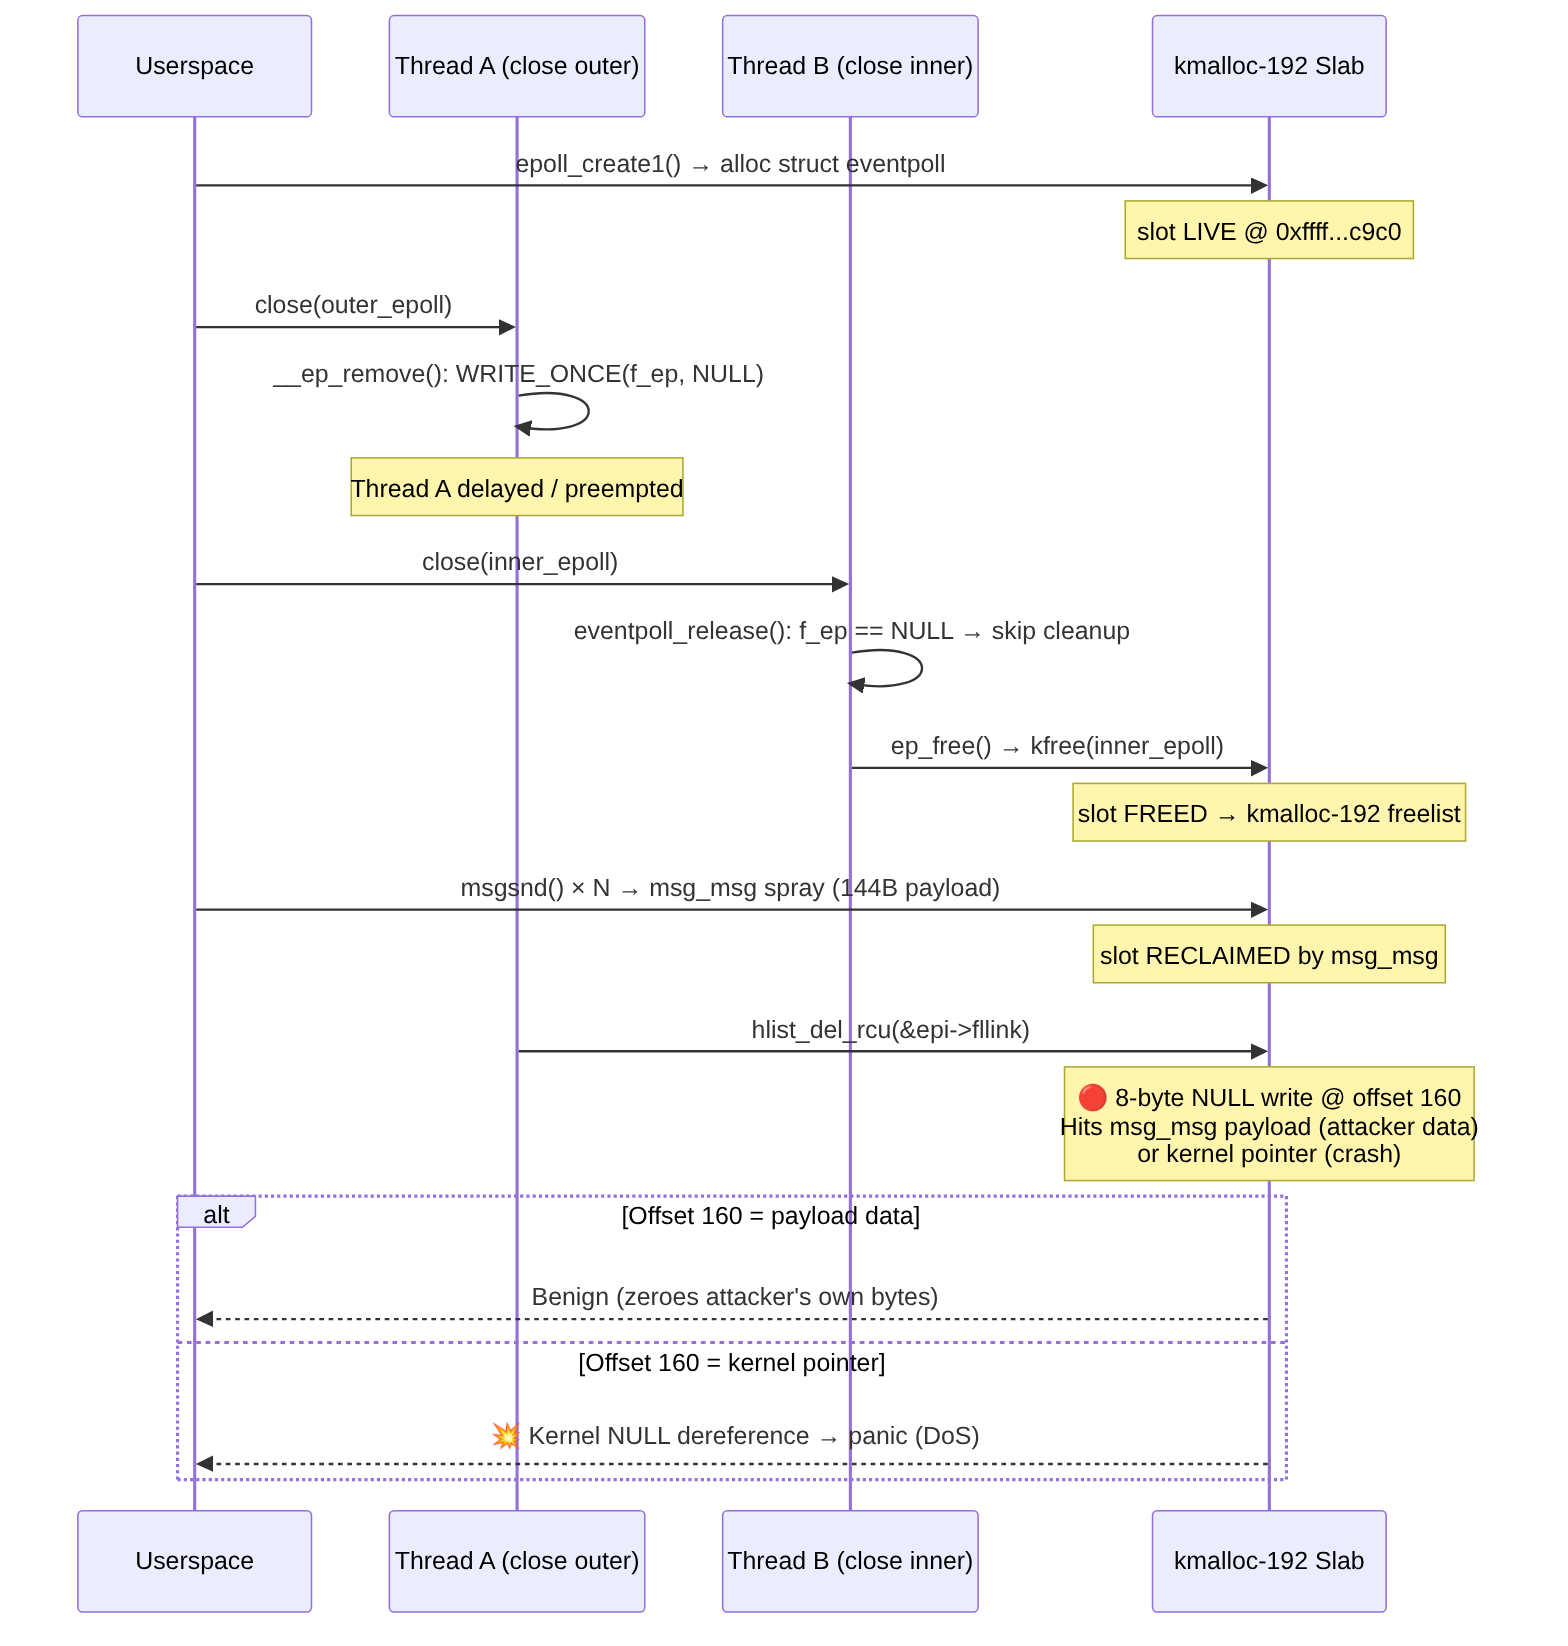
\includegraphics[width=\textwidth]{assets/diagram-02.png}
\caption{msg\_msg Reclaim Mechanics}
\end{figure}

\newpage

% ============================================================
% 21 DEAD ENDS
% ============================================================
\section{The 21 Dead Ends}

Four chains hypothesized, investigated, disproven --- each with killing evidence.

\begin{figure}[H]
\centering
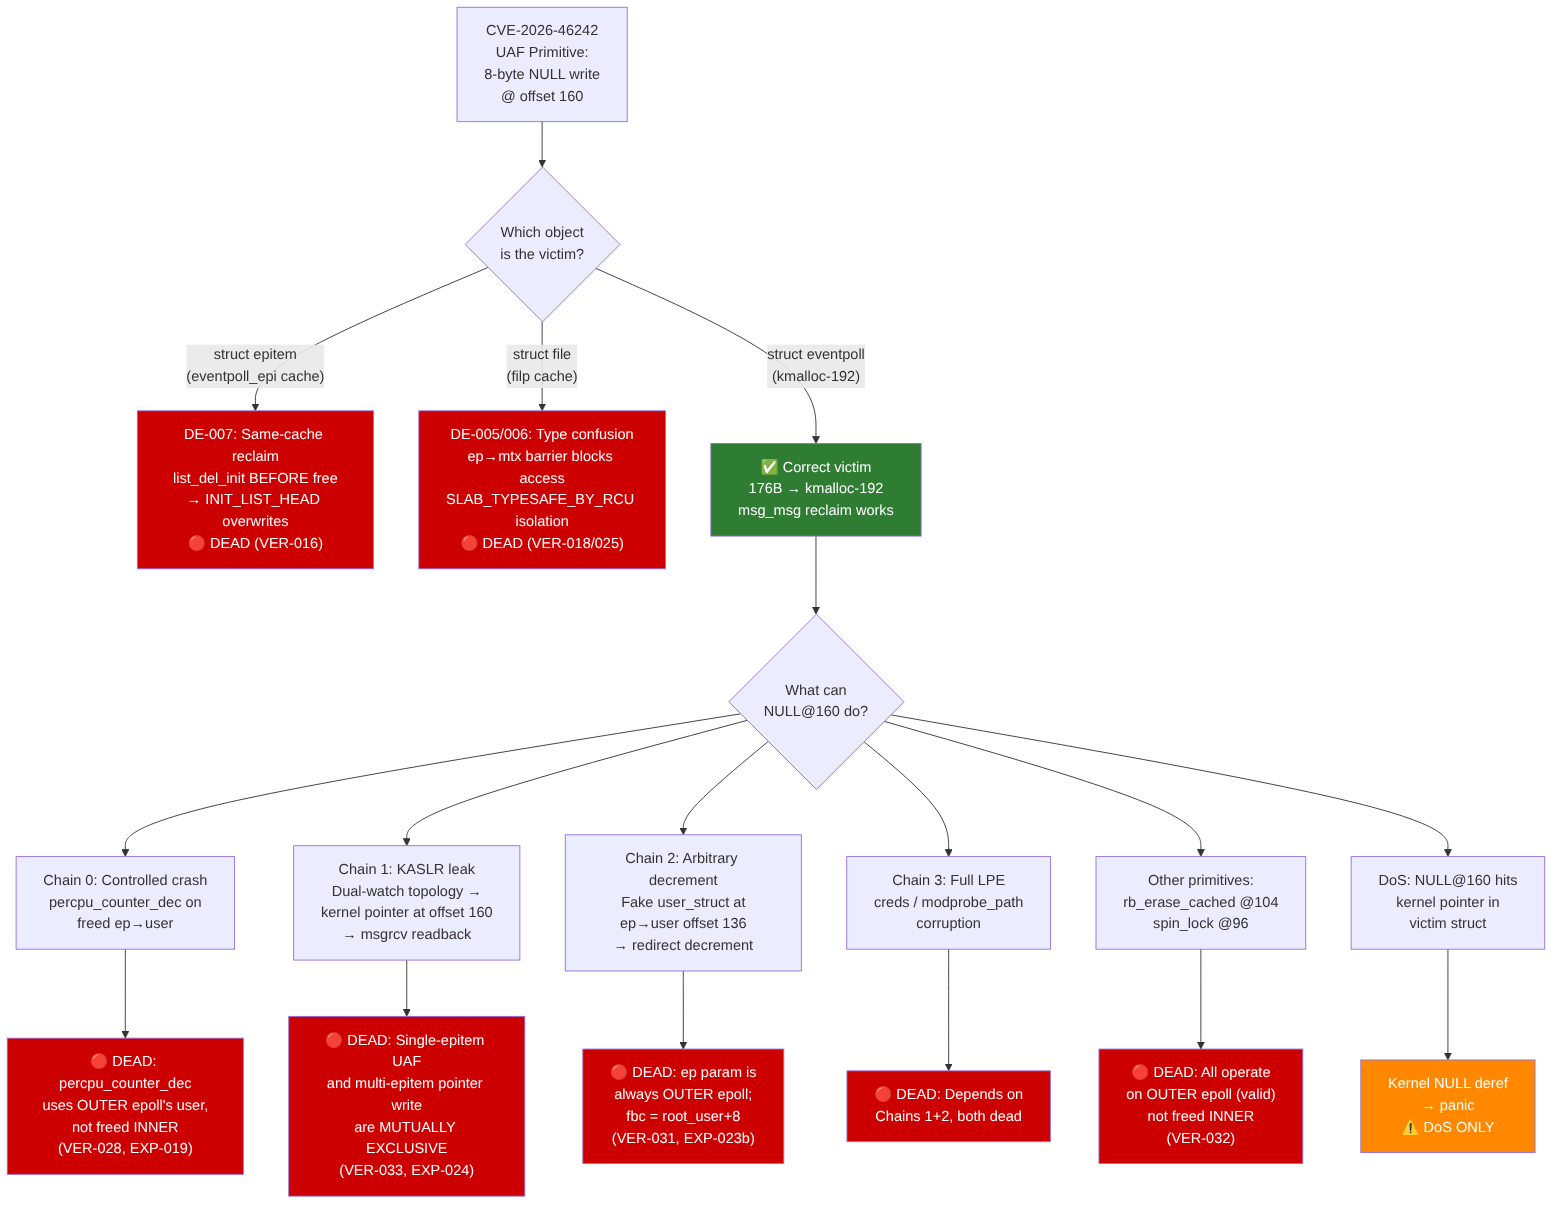
\includegraphics[width=\textwidth]{assets/diagram-04.png}
\caption{Exploitation Decision Tree}
\end{figure}

\subsubsection{Chain 0 --- Controlled Crash via \inlinecode{percpu\_counter\_dec}}
\textbf{Hypothesis:} Reclaim freed eventpoll with \texttt{msg\_msg} containing fake \texttt{user\_struct} at offset 136 $\to$ \texttt{\_\_ep\_remove()} calls \texttt{percpu\_counter\_dec(\&ep->user->epoll\_watches)} $\to$ deref attacker pointer.

\textbf{Killing (VER-028, EXP-019):} \texttt{percpu\_counter\_dec} uses \textbf{outer} eventpoll's \texttt{user} (valid), not freed inner. \texttt{ep} param always outer. Marker at offset 136 placed but never read.

\subsubsection{Chain 1 --- KASLR Leak via Dual-Watch}
\textbf{Hypothesis:} Two outer epolls watching inner $\to$ two epitems. Race fires $\to$ \texttt{hlist\_del\_rcu} writes \texttt{epi2} kernel address (not NULL) at offset 160 $\to$ read via \texttt{msgrcv} $\to$ KASLR defeated.

\textbf{Killing (VER-033, EXP-024):} UAF condition (single epitem: \texttt{f\_ep=NULL} path) and pointer-write condition (multi-epitem: \texttt{hlist\_del\_rcu} writes next node) are \textbf{mutually exclusive}. 2+ epitems $\to$ \texttt{WRITE\_ONCE(f\_ep,NULL)} never executes $\to$ lockless bypass never triggers $\to$ inner never freed $\to$ \texttt{hlist\_del\_rcu} writes to \textbf{live} memory. HW watchpoint: \texttt{ep\_free\_inner\_seen=False} at write.

\subsubsection{Chain 2 --- Arbitrary Decrement via Fake \inlinecode{user\_struct}}
\textbf{Hypothesis:} Fake \texttt{user\_struct} at known addr $\to$ overwrite \texttt{ep->user} (offset 136) via spray $\to$ \texttt{percpu\_counter\_dec} decs attacker's counter (\texttt{modprobe\_path} / creds).

\textbf{Killing (VER-031, EXP-023b):} Same as Chain 0. \texttt{percpu\_counter\_add\_batch} showed \texttt{fbc = root\_user+8} (outer epoll's user). \texttt{ep} never freed object.

\subsubsection{Chain 3 --- Full LPE}
\textbf{Hypothesis:} Chain 1 + Chain 2 $\to$ creds / \texttt{modprobe\_path} corruption.

\textbf{Killing:} Both prerequisites dead.

\subsubsection{Additional Dead Ends}

\begin{table}[H]
\centering
\caption{Additional Dead Ends}
\begin{tabularx}{\textwidth}{>{\bfseries\color{accent}}l X}
\toprule
\textbf{Path} & \textbf{Why Dead} \\
\midrule
\texttt{rb\_erase\_cached} arb write @104 & Operates on outer epoll's \texttt{rbr} (valid) \\
\texttt{spin\_lock\_irq} corrupt @96 & Operates on outer epoll's \texttt{lock} (valid) \\
\texttt{struct file} type confusion & \texttt{ep->mtx} blocks concurrent access to stale epitem \\
\texttt{pipe\_buffer} $\to$ \texttt{struct file} cross-cache & \texttt{SLAB\_TYPESAFE\_BY\_RCU} + size mismatch \\
\texttt{epitem} same-cache reclaim & \texttt{list\_del\_init} before \texttt{call\_rcu} --- corrupt doesn't survive \\
\texttt{snd\_timer\_user} reclaim & Different slab cache entirely \\
\texttt{eventpoll\_epi} $\to$ \texttt{kmalloc-128} merge & \texttt{SLAB\_ACCOUNT} prevents merge \\
\bottomrule
\end{tabularx}
\end{table}

\newpage

% ============================================================
% SCHEDULABILITY WALL
% ============================================================
\section{The Schedulability Wall}

Even with a useful primitive, race never fires without GDB.

\subsubsection{Natural Race Attempts}

\begin{table}[H]
\centering
\caption{Natural Race Attempts}
\begin{tabular}{lccc}
\toprule
\textbf{Experiment} & \textbf{Iterations} & \textbf{Hits} & \textbf{Optimizations} \\
\midrule
NAT-001 & 10,000 & \textbf{0} & Baseline, 2 CPUs \\
NAT-005 & 92,740 & \textbf{0} & \texttt{isolcpus=1}, 4MB cache eviction, 10-cycle delay steps, closed-loop calibration \\
\textbf{Total} & \textbf{102,740} & \textbf{0} & Best alignment: 1 cycle ($\sim$16 ns) at delay=2,360 \\
\bottomrule
\end{tabular}
\end{table}

\textbf{Root cause:}
\begin{enumerate}
  \item \texttt{cond\_resched()} at \texttt{eventpoll.c:888/903} = \textbf{no-op}: \texttt{dynamic\_cond\_resched} key = \texttt{FALSE} under \texttt{CONFIG\_PREEMPT\_DYNAMIC} default \texttt{PREEMPT\_VOLUNTARY}; \texttt{TIF\_NEED\_RESCHED} never set on pinned CPU (VER-035)
  \item \texttt{\_\_ep\_remove} = \textbf{zero} preemption points (disassembly)
  \item Vulnerable sequence runs atomically wrt scheduling
  \item Real window: $\sim$250--550 cycles ($\sim$125--275 ns @ 2 GHz) --- below scheduling granularity
\end{enumerate}

\begin{figure}[H]
\centering
\begin{mdframed}[backgroundcolor=cardbg,linecolor=fgmuted,linewidth=1pt,roundcorner=6pt,innerleftmargin=12pt,innerrightmargin=12pt,innertopmargin=10pt,innerbottommargin=10pt]
\noindent\textbf{Natural Race Hit Rate (QEMU TCG)}\\[0.5em]
\begin{tabular}{ll}
NAT-001:  0 / 10,000 \hspace{1em} (CI upper bound: 0.0384\%) & \color{fgmuted}#################### 0\% \\
NAT-005:  0 / 92,740 \hspace{1em} (extreme optimization) & \color{fgmuted}#################### 0\% \\
Combined: 0 / 102,740 & \color{fgmuted}#################### 0\% \\
95\% CI upper bound: < 0.003\% & \\
Required for exploit: $\ge$ 0.01\% (conservative) & \\
\multicolumn{2}{l}{\textbf{Race window:} WRITE\_ONCE(f\_ep,NULL) \textemdash\textemdash 250-550 cycles \textemdash\textemdash\textgreater UAF} \\
\multicolumn{2}{l}{Thread A writes \hspace{3em} Thread B must see NULL, free, and Thread A} \\
\multicolumn{2}{l}{then continues \hspace{3em} must resume in this window} \\
Scheduling granularity: \textasciitilde 4,000,000 cycles & \\
Race window: \textasciitilde 400 cycles & \\
Ratio: 1 : 10,000 & \\
Best alignment: 1 cycle error (\textasciitilde 16 ns) \hspace{1em} Still: 0 hits &
\end{tabular}
\end{mdframed}
\caption{Why 0/102,740 Is Conclusive}
\end{figure}

\begin{dangerbox}
\noindent\textbf{[HW] Hardware Caveat:} QEMU TCG doesn't model real cache-coherency latency, store buffer propagation, or asymmetric core clock drift. On physical ARM64 (Cortex-X4 3.2 GHz + Cortex-A520 1.8 GHz), hardware effects create natural phase shifts that \textit{could} widen the window. First-principles analysis says race is \textbf{physically viable} on real silicon --- but primitive stays capped at DoS regardless.
\end{dangerbox}

\newpage

% ============================================================
% WHY MITIGATIONS WORKED
% ============================================================
\section{Why Android's Mitigations Worked}

Even with 100\% reliable race on hardware, mitigation stack blocks escalation:

\subsection{Control-Flow Integrity}

\begin{table}[H]
\centering
\caption{Control-Flow Integrity}
\begin{tabularx}{\textwidth}{>{\bfseries\color{accent}}l X}
\toprule
\textbf{Mitigation} & \textbf{Blocks} \\
\midrule
\textbf{PAC} & Function ptrs cryptographically signed. Forging \texttt{f\_op->poll} $\to$ HW fault. \textbf{PACMAN} (MIT CSAIL '22) shows speculative oracles in userland, but unguided NULL-write lacks arbitrary read oracle for valid signatures. \\
\textbf{kCFI} & Clang validates 32-bit type hashes before indirect \texttt{blr}. Valid addr fails if hash mismatches. \\
\textbf{BTI} & Indirect branches must land on \texttt{bti c} landing pads. Random gadgets unreachable. \\
\bottomrule
\end{tabularx}
\end{table}

\subsection{Memory Safety}

\begin{table}[H]
\centering
\caption{Memory Safety}
\begin{tabularx}{\textwidth}{>{\bfseries\color{accent}}l X}
\toprule
\textbf{Mitigation} & \textbf{Blocks} \\
\midrule
\textbf{MTE} & 4-bit tags / 16-byte granule. Freed memory access with mismatched tag $\to$ sync HW fault. \textbf{TikTag} ('24) shows speculative tag leakage, but async multicore noise prevents reliable recovery in unguided race $\to$ stale UAF = immediate HW exception. \\
\textbf{SLAB\_TYPESAFE\_BY\_RCU} & \texttt{filp\_cachep} can't be reclaimed by different caches. \\
\textbf{SLAB\_ACCOUNT} & \texttt{eventpoll\_epi} fully isolated from generic kmalloc. \\
\bottomrule
\end{tabularx}
\end{table}

\subsection{Scheduling}

\begin{table}[H]
\centering
\caption{Scheduling}
\begin{tabularx}{\textwidth}{>{\bfseries\color{accent}}l X}
\toprule
\textbf{Mitigation} & \textbf{Blocks} \\
\midrule
\textbf{PREEMPT\_VOLUNTARY} & \texttt{\_\_ep\_remove} = 0 preemption points. Vulnerable seq runs atomically. \\
\textbf{No \texttt{cond\_resched}} & \texttt{dynamic\_cond\_resched} = FALSE; \texttt{TIF\_NEED\_RESCHED} never set on pinned CPUs. \\
\bottomrule
\end{tabularx}
\end{table}

x86\_64 bypassed KASLR/SMEP/SMAP/KPTI via AAR/JOP/ROP/\texttt{SWAPGS}. ARM64 adds PAC/BTI/kCFI/MTE/slab isolation --- and they held.

\newpage

% ============================================================
% LESSONS
% ============================================================
\section{Lessons \& Takeaways}

\begin{enumerate}
  \item \textbf{Vuln $\neq$ Exploit.} CVE-2026-46242 real, verified, mechanically reproducible. x86\_64 = root. Backported GKI 6.1 = kernel panic. Gap between \enquote{bug exists} and \enquote{bug exploitable} = the whole story. Stock GKI 6.1 never exposed (bug intro v6.4).

  \item \textbf{Mitigation stack works in depth.} No single mitigation killed it --- all contributed. PAC blocks ptr forgery, kCFI blocks indirect call hijack, SLAB blocks cross-cache, MTE detects stale access, PREEMPT\_VOLUNTARY closes scheduling window. Each layer removes options until nothing viable.

  \item \textbf{Negative results are signal.} 21 dead ends, 3 retractions, 0/102,740 hits = definitive: this is what vuln looks like when mitigations actually work. Too much research only publishes wins. Failures = signal.

  \item \textbf{Evidence discipline prevents bias.} Phase 3 adversarial review (EVO-009) found \textbf{every} prior race demo was GDB-assisted --- artificial preemption point absent in real kernel. Without ledger tracking \textit{how} claims were proven, this goes unnoticed. Track methodology, not just results.

  \item \textbf{Compiler changes break exploit portability.} Tier 1 failed initially: GCC 16 shifted every gadget vs Google's Clang. Same kernel version, same source, different binary layout. \texttt{target\_db.kxdb} must match exact executing binary.

  \item \textbf{Attack surface shifting to drivers.} Core subsystems well-mitigated $\to$ remaining surface = vendor drivers (GPU, camera, audio) often lacking same hardening. Vendor GPU drivers = deterministic page-level UAFs + direct physmem manipulation $\to$ sidestep PAC/BTI/kCFI without ptr forgery.
\end{enumerate}

\newpage

% ============================================================
% OPEN QUESTIONS
% ============================================================
\section{Open Questions}

DoS-only verdict for backported-vuln GKI 6.1.23 (stock GKI 6.1 unaffected). Open:

\begin{enumerate}
  \item \textbf{Physical ARM64 validation:} Race fire naturally on real silicon (Cortex-X4 + Cortex-A520)? First-principles says yes, but rate? 2-week HW timebox $\sim$1M iterations would settle.
  \item \textbf{Alt kmalloc-192 victims:} EXP-016 covered \texttt{fib6\_info}, \texttt{snd\_timer\_user}, \texttt{packet\_fanout}, \texttt{urb}, \texttt{wakeup\_source}. Other structs where NULL @160 corrupts something useful? Deep slab cross-ref on vuln GKI 6.1 builds?
  \item \textbf{Different kernel configs:} Assessment on \texttt{PREEMPT\_VOLUNTARY} + \texttt{PREEMPT\_DYNAMIC}=voluntary. \texttt{PREEMPT\_FULL} or vendor kernels add schedulable points in \texttt{\_\_ep\_remove}?
  \item \textbf{Data-only attacks:} Control-flow hijacking blocked by PAC/BTI/kCFI. Data-only path from fixed NULL write (8B, 0x0, offset 160, single write)? Constraint brutal, but data-only attacks surprise us.
\end{enumerate}

\begin{pullquote}
\noindent\textbf{[CHAT] Collaborate?} Vuln is public, repos linked, evidence chain documented. Fresh eyes on kmalloc-192 or scheduling could flip Tier 2 verdict. Ping me.
\end{pullquote}

\newpage

% ============================================================
% DISCLOSURE
% ============================================================
\section{Disclosure \& Attribution}

\begin{itemize}
  \item \textbf{Original Vuln \& Exploit:} Jaeyoung Chung, kernelCTF, \texttt{github.com/J-jaeyoung/bad-epoll}
  \item \textbf{Upstream Patch:} \texttt{a6dc643c693} (v6.11 / v7.1-rc1)
  \item \textbf{This Research:} Independent Tier 1 x86\_64 reproduction + original Tier 2 portability/mitigation study on deliberately backported-vuln Android 14 ARM64 GKI 6.1.23. Stock GKI 6.1 \textbf{NOT} affected (\texttt{58c9b016e128} absent); test kernel = base + cherry-pick \texttt{a1f93804449d}. No 0-days.
\end{itemize}

\begin{figure}[H]
\centering
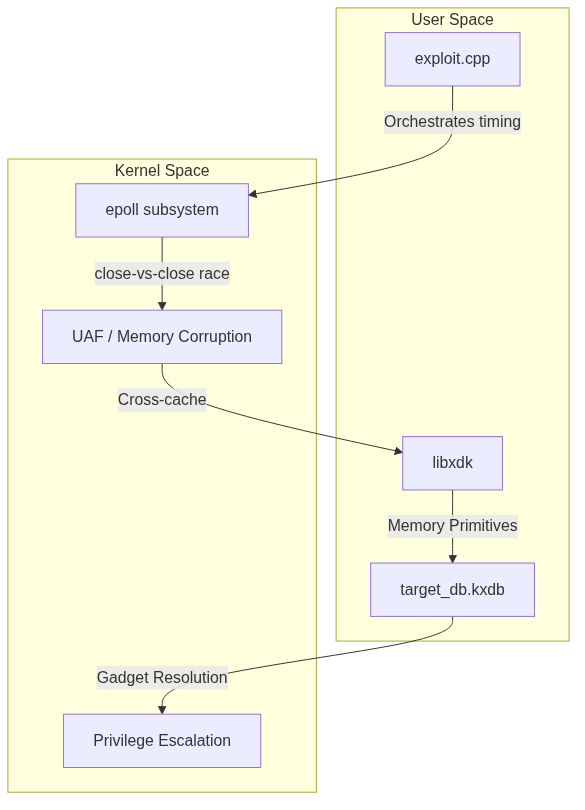
\includegraphics[width=0.95\textwidth]{assets/arch.png}
\caption{Architecture Map --- Userland to Kernel Escalation Flow}
\end{figure}

\begin{figure}[H]
\centering
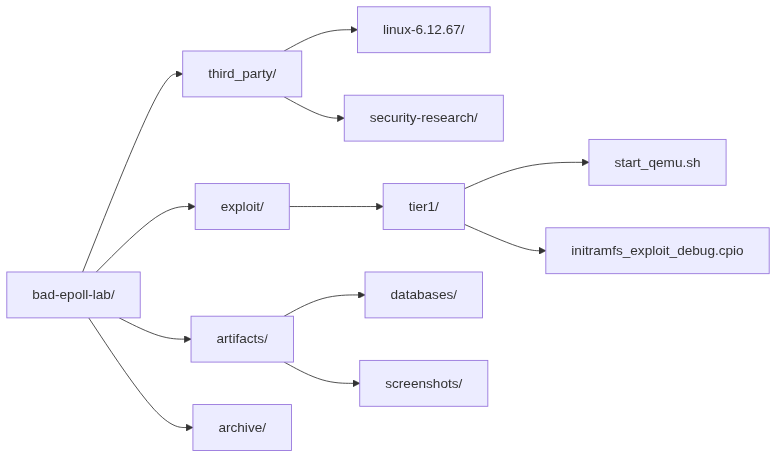
\includegraphics[width=0.7\textwidth]{assets/repo.png}
\caption{Repository Layout — Tier-1 (left) vs Tier-2 (right) separation}
\end{figure}

\appendix
\section{Verification Ledger — Summary (42 entries)}
\label{app:ver}
Full ledger at \texttt{tier2/docs/VERIFICATION\_LEDGER.md} and \texttt{knowledge/02\_projects/bad-epoll/02\_tier2/01\_evidence/}. Excerpt (VER-026/027/028/031/033/034/039 are load-bearing):

\begin{longtable}{>{\bfseries}l l p{7.2cm}}
\caption{Verification Ledger Excerpt} \\
\toprule
\textbf{ID} & \textbf{Status} & \textbf{Claim} \\
\midrule
\endfirsthead
\toprule
\textbf{ID} & \textbf{Status} & \textbf{Claim} \\
\midrule
\endhead
VER-026 & VERIFIED & Race proven via HW watchpoint: Thread A \texttt{WRITE\_ONCE(f\_ep,NULL)}, Thread B lockless bypass, Thread A \texttt{hlist\_del\_rcu} NULL@160 on freed object. \\
VER-027 & VERIFIED & \texttt{msg\_msg} 144B reclaims freed \texttt{eventpoll} (marker \texttt{0xdead...} @ offset 136). \\
VER-028 & VERIFIED & \texttt{percpu\_counter\_dec} uses OUTER epoll's user, not freed inner — Chain 0 dead. \\
VER-031 & VERIFIED & \texttt{fbc=root\_user+8} — arbitrary decrement dead. \\
VER-033 & VERIFIED & Single-epitem UAF vs multi-epitem pointer-write mutually exclusive — Chain 1 dead (retracts VER-029/030). \\
VER-034/039 & VERIFIED & NAT-001 (10k) + NAT-005 (92,740) = 0/102,740 natural hits. \\
VER-035 & VERIFIED & \texttt{cond\_resched} no-op, \texttt{\_\_ep\_remove} 0 preemption points. \\
\bottomrule
\end{longtable}
3 retracted (VER-010/029/030) kept visible with reasons.

\section{Dead Ends Register — 21 Entries}
\label{app:dead}
Full register at \texttt{tier2/docs/DEAD\_ENDS\_REGISTER.md} (also \texttt{knowledge/02\_projects/bad-epoll/02\_tier2/02\_analysis/}). All 21 mapped to killing VER/EXP; 4 chains + 7 additional paths listed in \S\ref{sec:deadends}.

\section{Experiment Index — NAT \& EXP}
\label{app:exp}
\texttt{tier2/docs/EXPERIMENT\_INDEX.md} (\texttt{knowledge/02\_projects/bad-epoll/02\_tier2/01\_evidence/}):

\begin{tabular}{lll}
\toprule
\textbf{ID} & \textbf{Iters} & \textbf{Outcome} \\
\midrule
NAT-001 & 10,000 & 0 hits, baseline 2 CPUs \\
NAT-005 & 92,740 & 0 hits, isolcpus+eviction+sweeper, best align 1 cyc \\
EXP-015/018/019 & — & GDB race + msg\_msg reclaim, Chain 0 killing \\
EXP-023b/024 & — & Chain 1/2 mutual exclusion \\
\bottomrule
\end{tabular}

\section{Glossary}
\label{app:gloss}
\begin{tabular}{lp{11cm}}
\toprule
\textbf{Term} & \textbf{Meaning} \\
\midrule
UAF & Use-After-Free — free then use via dangling pointer \\
SLAB & Kernel allocator; \texttt{kmalloc-192}, \texttt{eventpoll\_epi} dedicated, \texttt{SLAB\_ACCOUNT}/\texttt{TYPESAFE\_BY\_RCU} isolation \\
KASLR & Kernel ASLR — base randomization, bypass via AAR leak \\
PAC/BTI/kCFI & ARM64 CFI: pointer signing, landing pads, type hashes \\
MTE & Memory Tagging — 4-bit tags/16B granule, stale access = fault \\
PREEMPT\_VOLUNTARY & Voluntary preemption — \texttt{\_\_ep\_remove} has 0 points \\
\bottomrule
\end{tabular}

\section{Repositories \& Reproducibility}
\label{app:repo}
\begin{tabular}{ll}
\toprule
\textbf{Repo} & \textbf{URL / Commit} \\
\midrule
Tier-1 & \texttt{github.com/Aayushbankar/bad-epoll-lab} @ \texttt{publish/clean-and-writeup-2026-08-29} \\
Tier-2 & \texttt{github.com/Aayushbankar/bad\_epoll\_ab\_tier2} @ \texttt{main} \\
Base GKI & \texttt{7e35917775b8} (stock NOT vuln) + backport \texttt{a1f93804449d} (vuln test) \\
Artifacts & \texttt{tier2/android/artifacts/Image}, \texttt{vmlinux}, \texttt{System.map}, \texttt{initramfs.cpio} \\
Evidence & \texttt{tier2/evidence/2026-07-*} (hashes, qemu logs, GDB traces) \\
\bottomrule
\end{tabular}
Rebuild: see \S\ref{sec:env}. No Mali hunt content included — out of scope for this Bad Epoll dossier (see separate \texttt{cve-primitive-hunt} KB).

\newpage

% ============================================================
% ABOUT AUTHOR
% ============================================================
\section{About the Author}

\noindent\textbf{Aayush Bankar} --- Cybersecurity Analyst @ CypherMatrix.

Research workflow augmented by AI-assisted agentic coding tools (local LLM orchestration) for code comprehension, hypothesis generation, evidence organization --- all engineering decisions \& runtime evidence manually verified. AI workflow documented in Tier 1 Final Writeup.

\vspace{1.5em}
\noindent\textbf{Connect:}
\githubicon\ \href{https://github.com/Aayushbankar}{github.com/Aayushbankar} $\cdot$
\linkedinicon\ \href{https://linkedin.com/in/aayushbankar}{linkedin.com/in/aayushbankar}

\vspace{3em}
\begin{center}
{\color{fgmuted}\textit{Thanks for reading. If you work in kernel exploitation, Android security, or mitigation engineering --- perspective appreciated, especially on open questions. Best outcomes come from collaborative scrutiny, not solo claims.}}
\end{center}

\end{document}